\documentclass[letterpaper, 10pt, conference]{ieeeconf}
\IEEEoverridecommandlockouts \overrideIEEEmargins
\usepackage{amsmath,amssymb,url}
\usepackage{graphicx,subfigure}
\usepackage{color}
\usepackage{siunitx}
%\usepackage[hidelinks]{hyperref}
\usepackage{cleveref}
\usepackage{tikz}

\newcommand{\norm}[1]{\ensuremath{\left\| #1 \right\|}}
\newcommand{\abs}[1]{\ensuremath{\left| #1 \right|}}
\newcommand{\bracket}[1]{\ensuremath{\left[ #1 \right]}}
\newcommand{\braces}[1]{\ensuremath{\left\{ #1 \right\}}}
\newcommand{\parenth}[1]{\ensuremath{\left( #1 \right)}}
\newcommand{\ip}[1]{\ensuremath{\langle #1 \rangle}}
\newcommand{\tr}[1]{\mbox{tr}\ensuremath{\negthickspace\bracket{#1}}}
\newcommand{\deriv}[2]{\ensuremath{\frac{\partial #1}{\partial #2}}}
\newcommand{\G}{\ensuremath{\mathsf{G}}}
\newcommand{\SO}{\ensuremath{\mathsf{SO(3)}}}
\newcommand{\T}{\ensuremath{\mathsf{T}}}
\renewcommand{\L}{\ensuremath{\mathsf{L}}}
\newcommand{\so}{\ensuremath{\mathfrak{so}(3)}}
\newcommand{\SE}{\ensuremath{\mathsf{SE(3)}}}
\newcommand{\se}{\ensuremath{\mathfrak{se}(3)}}
\renewcommand{\Re}{\ensuremath{\mathbb{R}}}
\newcommand{\Sph}{\ensuremath{\mathsf{S}}}
\newcommand{\aSE}[2]{\ensuremath{\begin{bmatrix}#1&#2\\0&1\end{bmatrix}}}
\newcommand{\ase}[2]{\ensuremath{\begin{bmatrix}#1&#2\\0&0\end{bmatrix}}}
\newcommand{\D}{\ensuremath{\mathbf{D}}}
\newcommand{\pair}[1]{\ensuremath{\left\langle #1 \right\rangle}}
\newcommand{\met}[1]{\ensuremath{\langle\!\langle #1 \rangle\!\rangle}}
\newcommand{\Ad}{\ensuremath{\mathrm{Ad}}}
\newcommand{\ad}{\ensuremath{\mathrm{ad}}}
\newcommand{\g}{\ensuremath{\mathfrak{g}}}
\DeclareMathOperator*{\argmin}{arg\,min}

\newcommand\encircle[1]{%
  \tikz[baseline=(X.base)] 
    \node (X) [draw, shape=circle, inner sep=0] {#1};}


\title{\LARGE \bf Variational Symplectic Accelerated Optimization on Lie Groups}

%\author{Taeyoung Lee%\authorrefmark{1}%
    %\thanks{Taeyoung Lee, Mechanical and Aerospace Engineering, George Washington University, Washington, DC 10051 {\tt tylee@gwu.edu}}%
    %%\thanks{\textsuperscript{\footnotesize\ensuremath{*}}This research has been supported in part by NSF under the grant CNS-1837382.}%
%}


\newcommand{\RomanNumeralCaps}[1]{\textup{\uppercase\expandafter{\romannumeral#1}}}
\newcommand{\RI}{\RomanNumeralCaps{1}}
\newcommand{\RII}{\RomanNumeralCaps{2}}
\newcommand{\RIII}{\RomanNumeralCaps{3}}

\newcommand{\EditTL}[1]{{\color{red}\protect #1}}
\renewcommand{\EditTL}[1]{{\protect #1}}


\newtheorem{definition}{Definition}
\newtheorem{lem}{Lemma}
\newtheorem{prop}{Proposition}
\newtheorem{remark}{Remark}

\graphicspath{{./figs/}}

%\color{white}\pagecolor{black}

\begin{document}
\allowdisplaybreaks


\maketitle \thispagestyle{empty} \pagestyle{empty}

\begin{abstract}
\end{abstract}

\section{Introduction}

\section{Extended Lagrangian Mechanics}

This section presents Lagrangian mechanics for non-autonomous systems on a Lie group. 
It is referred to as \textit{extended} Lagrangian mechanics as the variational principle is extended to include reparamerization of time~\cite{MarWesAN01}.
These are developed in both of continuous-time and discrete-time formulations, and the latter is often referred to as \textit{Lie group variational integrator}~\cite{LeeLeoCMAME07}.
They will be utilized in accelerated optimization with Bregman Lagrangian in the next section.

Consider  an $n$-dimensional Lie group $\G$.
Let $\g$ be the lie algebra, or the tangent space at the identity, i.e., $\g = \T_e\G$.
The tangent bundle of the group is identified with $\T\G \simeq \G\times \g$ via left trivialization.
More specifically, let $\L:\G\times\G\rightarrow\G$ be the left action defined such that $\L_g h = gh$ for $g,h\in\G$.
For any $v\in\T_g\G$, there exists $\xi\in\g$ such that $v =\T_e\L_g \xi=g\xi$.
Utilizing this, the kinematics equation can be written as
\begin{align}
    \dot g = g\xi. \label{eqn:g_dot}
\end{align}
Further, suppose $\g$ is equipped with an inner product $\pair{\cdot, \cdot}$, which is extended to the corresponding inner product on $\T_g\G$ through the left trivialization.
For any $v,w\in\T_g\G$, we have $\pair{w,v}_{\T_g\G} = \pair{ \T_g \L_{g^{-1}} v, \T_g \L_{g^{-1}} w}_\g$. 
Considering the inner product as a pairing between a tangent vector and a cotangent vector, we identify $\g\simeq \g^*$ and $\T_g \G \simeq \T^*_g \G\simeq G\times \g^*$.
Throughout this paper, the pairing is also denoted by $\cdot$.
Let $\mathbf{J}:\g\rightarrow\g^*$ be defined such that $\pair{\mathbf{J}(\xi),\zeta}$ is positive-definite and symmetric as a bilinear form of $\xi,\zeta\in\g$.
Define the metric $\met{\cdot,\cdot}:\g\times\g\rightarrow\Re$ with $\met{\xi,\zeta} = \pair{\mathbf{J}(\xi),\zeta}$.
This serves as a left-invariant Riemmanian metric on $\G$.
Also $\|\xi\|^2 = \met{\xi,\xi}$ for any $\xi\in\g$.
The adjoint operator is denoted by $\Ad_g:\g\rightarrow\g$, and the ad operator is denoted by $\ad_\xi:\g\rightarrow\g$. See, for example~\cite{MarRat99} for detailed preliminaries. 

\subsection{Continuous-Time Extended Lagrangian Mechanics}

Consider a non-autonomous Lagrangian $L(t,g,\xi):\Re\times\G\times\g\rightarrow \Re$ on the \textit{extended state space} including the space of time.
The corresponding \textit{extended path space} is composed of the curves $(c_t(a),c_g(a))$ on $\Re\times \G$ parameterized by $a>0$.
To ensure that the reparameterized time increases monotonically, we require $c'_t(a) > 0$. 
For a given interval of time $[t_0,t_f]$, the equivalent interval $[a_0,a_f]$ of $a$ is chosen such that $t_0=c_t(a_0)$ and $t_f=c_t(a_f)$.
For any path $(c_t(a),c_g(a))$ over $[a_0,a_f]$ in the extended space, the \textit{associated curve} is defined by
\begin{align}
    g(t) = c_g(c_t^{-1}(t)),\label{eqn:ac}
\end{align}
on $\G$ over $[t_0,t_f]$.
For a given extended path, define the \textit{extended action integral} as
\begin{align}
    \mathfrak{G}(c_t,c_g) = \int_{t_0}^{t_f} L(t,g,\xi)\bigg|_{g(t) = c_g(c_t^{-1}(t))} dt,\label{eqn:AI}
\end{align}
where the Lagrangian is evaluated through the associated curve \eqref{eqn:ac}.

Taking the variation of $\mathfrak{G}$ with respect to the extended path, we obtain the Euler-Lagrange equation according to the variational principle in the extended phase space. 
As discussed in~\cite[Sec. 4.2.2]{MarWesAN01}, the resulting Euler-Lagrangian equations depends only on the associated curve \eqref{eqn:ac}, not on the extended path $(c_t,c_g)$ itself, and the variational principle does not dictate how the curve should be reparameterized. 

Further, the resulting Euler-Lagrangian equation share the exactly same form as (unextended) Lagrangian mechanics for the associated curve. 
As such, the Euler-Lagrange equation for non-autonomous Lagrangian $L(t,g,\xi):\Re\times\G\times\g\rightarrow \Re$ can be written as
\begin{align}
    \frac{d}{dt}\!\parenth{\deriv{L}{\xi}} - \ad^*_\xi \deriv{L}{\xi} - \T^*_e \L_g (\D_g L) = 0, \label{eqn:EL}
\end{align}
where $\D_g$ stands for the differential with respect to $g$ (see~\cite[Sec. 8.6.3]{LeeLeo17} for derivation of the above equation for autonomous Lagrangian).

Introducing the Legendre transform $\mu = \deriv{L}{\xi} \in\g^*$, and assuming that it is invertible, the Euler-Lagrange equation can be rewritten into
\begin{align}
    \dot \mu - \ad^*_{\xi} \mu - \T^*_e \L_g (\D_g L) = 0. \label{eqn:HE}
\end{align}

\subsection{Extended Lie Group Variational Integrator}

Variational integrators are geometric numerical integration schemes interpreted as discrete-time mechanics, and they are constructed by discretizing the variational principle for Lagrangian mechanics~\cite{MarWesAN01}.
The solutions of variational integrators are symplectic and they preserve any symmetry according to the discrete analogue of Nother's theorem.
As such, they provide long-term structural stability in numerical simulation. 
For Lagrangian mechanics evolving on a Lie group, the corresponding Lie group variational integrators have been presented in~\cite{Leo04,Lee08,LeeLeoCMAME07}.

Here, we develop extended Lie group variational integrators by discretizing the extended variational principle presented above, by following the general framework of~\cite{MarWesAN01}.
The \textit{extended discrete path space} is composed of the sequence $\{(t_k, g_k)\}_{k=0}^N$ on $\Re\times\G$, satisfying $t_{k+1}>t_k$.
Next, the discrete kinematics equation is chosen as
\begin{align}
    g_{k+1} = g_k f_k, \label{eqn:gkp}
\end{align}
for $f_k \in\G$ representing the relative update over a single timestep. 
The discrete Lagrangian $L_d(t_k, t_{k+1}, g_k, f_k): \Re\times\Re\times\G\times\G\rightarrow \Re$ is chosen such that the following \textit{extended discrete action sum}
\begin{align}
    \mathfrak{G}_d(\{(t_k, g_k)\}_{k=0}^N) = \sum_{k=0}^{N-1} L_d(t_k, t_{k+1}, g_k, f_k), \label{eqn:Gd}
\end{align}
approximates \eqref{eqn:AI}. 
Now the discrete Euler-Lagrange equations can be developed according to the variational principle as follows.

\begin{prop}
    The discrete path of $\{(g_k,f_k)\}_{k=0}^{N-1}$ extremizing \eqref{eqn:Gd} with fixed end point satisfies the following discrete Euler-Lagrange equation, or the extended Lie group variational integrator.
    \begin{gather}
        \T^*_e\L_{g_k}(\D_{g_k} L_{d_k})- \Ad^*_{f_k^{-1}} (\T^*_e\L_{f_k}(\D_{f_k} L_{d_k}))\nonumber \\
        + \T^*_e\L_{f_{k-1}}(\D_{f_{k-1}} L_{d_{k-1}}) =0,\label{eqn:DEL}\\
        \D_{t_k} L_{d_{k-1}} + \D_{t_k} L_{d_k} = 0, \label{eqn:DELt}
    \end{gather}
    along with \eqref{eqn:gkp}.
\end{prop}
\begin{proof}
    From \eqref{eqn:gkp},
    \begin{align*}
        \delta f_k = - g_k^{-1}( \delta g_k ) g_k^{-1} g_{k+1} + g_k^{-1}\delta g_{k+1}.
    \end{align*}
    Since $\delta g_k$ can be written as $\delta g_k = g_k \eta_k $ for $\eta_k\in \g$, 
    \begin{align*}
        \delta f_k = - \eta_k f_k +f_k \eta_{k+1}.
    \end{align*}
    Or equivalently, 
    \begin{align}
        f_k^{-1}\delta f_k = -\Ad_{f_k^{-1}} \eta_k + \eta_{k+1}.\label{eqn:del_fk}
    \end{align}

    Take the variation of \eqref{eqn:Gd} and substitute \eqref{eqn:del_fk} to obtain
    \begin{align*}
        \delta \mathfrak{G}_d  = \sum_{k=0}^{N-1}
        & \T^*_e\L_{g_k}(\D_{g_k} L_{d_k}) \cdot \eta_k \\
        & + \T^*_e\L_{f_k}(\D_{f_k} L_{d_k}) \cdot (-\Ad_{f_k^{-1}} \eta_k + \eta_{k+1}) \\
        & + \D_{t_k} L_{d_k}\cdot \delta t_k + \D_{t_{k+1}} \D_{d_k}\cdot \delta t_{k+1}.
    \end{align*}
    Since the endpoints are fixed, we have $\eta_0=0$ and $\delta t_0 = 0$.
    Therefore in the above expression, the range of summation for the terms paired with $\eta_k$ and $\delta t_k$ can be reduced to $1\leq k\leq N-1$. 
    Also, using $\eta_N=0$ and $\delta t_N=0$, for the other terms paired with $\eta_{k+1}$ and $\delta t_{k+1}$, the subscript can be reduced by one for the summation over the same range.
    Therefore, 
    \begin{align*}
        \delta \mathfrak{G}_d  = \sum_{k=1}^{N-1}
        & \big\{ \T^*_e\L_{g_k}(\D_{g_k} L_{d_k})- \Ad^*_{f_k^{-1}} (\T^*_e\L_{f_k}(\D_{f_k} L_{d_k})) \\
        & + (\T^*_e\L_{f_{k-1}}(\D_{f_{k-1}} L_{d_{k-1}})) \big\} \cdot \eta_{k} \\
        & + \{ \D_{t_k} L_{d_k} + \D_{t_{k}} \D_{d_{k-1}} \} \delta t_k.
    \end{align*}
    According to the variational principle, $\delta\mathfrak{G}_d = 0$ for any $\eta_k$ and $\delta t_k$, which yields \eqref{eqn:DEL} and \eqref{eqn:DELt}.
\end{proof}
The most notable difference against the continuous-time counterpart is that in addition to the discrete Euler-Lagrange equation \eqref{eqn:DEL}, we have the additional equation \eqref{eqn:DELt} for the evolution of the discrete time. 
This is because the discrete action sum $\mathfrak{G}_d$ depends on the complete extended path $\{(t_k,g_k)\}_{k=1}^N$.
Whereas the action $\mathfrak{G}$ in the continuous-time formulation is a function of the associated curve \eqref{eqn:ac} only.

The evolution of the discrete time is associated with the energy.
Let the discrete energies be
\begin{align}
    E^+_k &= - \D_{t_{k+1}} L_{d_k},\label{eqn:Ep}\\
    E^-_k &= \D_{t_{k}} L_{d_k}.\label{eqn:Em}
\end{align}
Then, \eqref{eqn:DELt} can be rewritten as
\begin{align}
    E^+_{k-1} = E^-_k,\label{eqn:DELE}
\end{align}
which reflects the evolution of the discrete energy.

In case the discrete Lagrangian is time-invariant so that $L_d(t_k,t_{k+1},g_k,f_k) =  L_d(t_k+s,t_{k+1}+s,g_k,f_k)$ for any $s$, 
we have $\D_{t_k}L_{d_k} + \D_{t_{k+1}}L_{d_k}=0$, or equivalently $E^-_k = E^+_k$. 
Combined with \eqref{eqn:DELE}, this yields $E_{k-1}^+ = E_k^+$ and $E_{k-1}^-=E_k^-$, which shows the conservation of discrete energy for autonomous Lagrangian systems. 

To implement \eqref{eqn:DEL} and \eqref{eqn:DELt} as a numerical integrator, it is more convenient to introduce the \textit{extended discrete Legendre transform}, $\mathbb{F}^\pm L_{d_k}: \Re\times\Re \times \G \times \G \rightarrow \Re\times \Re\times\G\times\g^*$ as
\begin{align}
    \mathbb{F}^+ L_{d_k} (t_k,t_{k+1}, g_k,f_k) & = (t_{k+1}, E_{k+1}, g_{k+1}, \mu_{k+1}),\\
    \mathbb{F}^- L_{d_k} (t_k,t_{k+1}, g_k,f_k) & = (t_k, E_k, g_{k}, \mu_{k}).
\end{align}
where
\begin{align}
    \mu_k & = -\T^*_e\L_{g_k}(\D_{g_k} L_{d_k})+ \Ad^*_{f_k^{-1}} (\T^*_e\L_{f_k}(\D_{f_k} L_{d_k})),\label{eqn:muk}\\
    \mu_{k+1} & = \T^*_e\L_{f_k} (\D_{f_k} L_{d_k}),\label{eqn:mukp}
\end{align}
and $E_{k+1}$ and $E_k$ are given by \eqref{eqn:Ep} and \eqref{eqn:Em}, respectively. 

The resulting discrete flow map is constructed by $\mathbb{F}^+L_{d_k} \circ (\mathbb{F}L_{d_k})^{-1}$. 
More specifically, for given $(t_k, E_k, g_k, \mu_k)$, \eqref{eqn:Em} and \eqref{eqn:muk} are solved together for $t_{k+1},f_k$ with the constraint $t_{k+1}>t_k$.
Then, $(E_{k+1}, g_{k+1},\mu_{k+1})$ are computed by \eqref{eqn:Ep}, \eqref{eqn:gkp}, and \eqref{eqn:mukp}, respectively.
This yields the discrete flow map $(t_k, E_k, g_k, \mu_k)\rightarrow(t_{k+1}, E_{k+1}, g_{k+1}, \mu_{k+1})$ consistent with \eqref{eqn:DEL} and \eqref{eqn:DELt}.
While the flow map is described by $E$ for convenience, the initial value of $E_0$ is often selected by choosing the initial timestep $h_0$ and calculating the corresponding value of $E_0$ through \eqref{eqn:Em}.
This inherits the desirable properties of variational integrators, and the group structure is also preserved through \eqref{eqn:gkp}.

\section{Bregman Lagrangian Systems on $\G$}

\newcommand{\obj}{\mathsf{f}}

Let $\obj:\G\rightarrow\Re$ be a real-valued smooth function on $\G$.
We focus on the optimization problem:
\begin{align}
    \min_{g\in\G} \obj (g).
\end{align}
Variational accelerated optimization scheme for the above problem has been presented in~\cite{tao2020variational}, where the Nesterov accelerated gradient (NAG) descent on a finite-dimensional vector space is intrinsically generalized to a Lie group. 
In this section, we consider an intrinsic formulation of the Bregman Lagrangian dynamics~\cite{wibisono2016variational}, which encloses a large class of accelerated optimization scheme, including NAG.
More importantly, it guarantees polynomial convergence rates up to an arbitrary order.

\subsection{Continuous-Time Bregman Dynamics}

The Bregman Lagrangian $L(t,g,\xi):\Re\times\G\times\g\rightarrow$ is given by
\begin{align}
    L(t,g,\xi) = \frac{t^{\lambda p+1}}{2p} \|\xi\|^2 - C p t^{(\lambda+1)p-1} \obj (g),\label{eqn:BL}
\end{align}
for $p, C>0$, and $\lambda\geq 1$.
When applied to $\G=\Re^n$ with $\lambda=1$, this is a special case of Bregman Lagrangian~\cite{wibisono2016variational}, and it recovers the continuous-time limit of Nesterov's accelerated minor descent with $p=2$~\cite{nesterov2005smooth}.
Also, in case $p = 3$, it corresponds to the continuous-time limit of Nesterov’s accelerated cubic-regularized Newton’s method~\cite{nesterov2008accelerating}.
When $\G$ is considered as a Riemannian manifold, this corresponds to the $p$-Bregman Lagrangian in~\cite{duruisseaux2021variational}.
The additional term $\lambda$ has been introduced in~\cite{alimisis2020continuous}, and it accounts the curvature of the manifold. 

Let the left-trivialized derivative of the objective function be
\begin{align}
    \nabla_\L \obj(g) = \T_e^*\L_g (\D_g \obj(g)).\label{eqn:grad}
\end{align}
According to \eqref{eqn:EL}, the Euler-Lagrange equations are obtained as follows.
\begin{prop}\label{prop:EL_Breg}
    The Euler-Lagrange equations corresponding to the Bregman Lagrangian \eqref{eqn:BL} are given by
    \begin{align}
        \frac{d \mathbf{J}(\xi)}{dt} + \frac{\lambda p+1}{t}\mathbf{J}(\xi) - \ad^*_\xi \mathbf{J}(\xi)
        + Cp^2 t^{p-2} \nabla_\L \obj (g) =0, \label{eqn:EL_Breg}
    \end{align}
    and \eqref{eqn:g_dot}. 
    Further, the corresponding continuous flow locally converges to the minimizer $g^*$ of $\obj$ with the rate given by
    \begin{align}
        \obj(g(t)) - \obj(g^*) \in \mathcal{O}(t^{-p}),
    \end{align}
    when $\obj$ is geodesically convex. 
\end{prop}
\begin{proof}
    We have
    \begin{align*}
        \deriv{L}{\xi} & = \frac{t^{\lambda p+1}}{p}\mathbf{J}(\xi)
    \end{align*}
    Substituting this into \eqref{eqn:EL} and using \eqref{eqn:grad}, 
    \begin{gather*}
        \frac{t^{\lambda p+1}}{p}\frac{d \mathbf{J}(\xi)}{dt} + \frac{(\lambda p+1)t^{\lambda p}}{p}\mathbf{J}(\xi) -\frac{t^{\lambda p+1}}{p} \ad^*_\xi \mathbf{J}(\xi) \\
        + Cpt^{(\lambda +1)p-1} \nabla_\L \obj(g) =0.
    \end{gather*}
    Dividing both sides by $\frac{t^{\lambda p+1}}{p}$ yields \eqref{eqn:EL_Breg}.
    The convergence property is established by~\cite[Theorem 3.2]{duruisseaux2021variational}.
\end{proof}

Therefore, the optimization problem on $\G$ can be addressed by numerically integrating \eqref{eqn:EL_Breg} from an initial guess. 
However, it has been discovered that a naive discretization is not able to match the polynomial convergence rate~\cite{wibisono2016variational}.
Here we have additional computational requirements that the optimal solution lies in the Lie group.

These two challenges can be addressed by the Lie group variational integrator, 
as their structure-preserving properties provide long-term numerical stabilities, and also the group structures are conserved. 
In the subsequent section, we develop Lie group variational integrators for the Bregman Lagrangian system. 

\subsection{Lie Group Variational Integrator for Bregman Dynamics}

Let $h_k = t_{k+1}- t_k$ and $t_{k,k+1} = t_k + h_k/2$.  
We consider the following form of the discrete Lagrangian
\begin{align}
    L_d(t_k, t_{k+1}, g_k, f_k ) & = \frac{\phi(t_{k,k+1}) }{h_k} T_d(f_k) -\frac{h_k}{2} \theta(t_k) \obj (g_k)\nonumber \\
                                 & \quad -\frac{h_k}{2} \theta(t_{k+1}) \obj (g_kf_k), \label{eqn:Ld}
\end{align}
where $T_d(f_k):\G\rightarrow\Re$ is chosen such that it approximate $T(f_k) \approx h_k^2 \|\xi_k \|^2/2$, and $\phi,\theta:\Re\rightarrow\Re$ are 
\begin{align}
    \phi(t) & = \frac{t^{\lambda p +1}}{p},\\
    \theta(t) & = C p t^{(\lambda+1)p-1}.
\end{align}
The corresponding variational integrators are presented as follows. 
\begin{prop}\label{prop:DEL_Breg}
    The discrete-time Euler-Lagrange equation, or the Lie group variational integrator for the Bregman Lagrangian corresponding to \eqref{eqn:Ld} are given by
\begin{align}
    \mu_k & =  \frac{\phi_{k,k+1}}{h_k}\Ad^*_{f_k^{-1}} (\T^*_e\L_{f_k}(\D_{f_k} T_{d_k})) + \frac{h_k\theta_k}{2} \nabla_L \obj_k, \label{eqn:muk_Breg}\\
    \mu_{k+1} & = \Ad^*_{f_k}( \mu_k - \frac{h_k\theta_k}{2} \nabla_L\obj_k ) -\frac{h_k\theta_{k+1}}{2} \nabla_\L \obj_{k+1}, \label{eqn:mukp_Breg}\\
    E_{k} & = \frac{\phi'_{k,k+1}}{ 2 h_k} T_{d_k} -\frac{h_k\theta'_{k}}{2} \obj_{k} \nonumber\\\
          & \quad + \frac{\phi_{k,k+1}}{h_k^2}T_{d_k} + \frac{\theta_k}{2}\obj_k + \frac{\theta_{k+1}}{2}\obj_{k+1}, \label{eqn:Ek_Breg}\\
    E_{k+1} & = -\frac{\phi'_{k,k+1}}{ 2 h_k} T_{d_k} +\frac{h_k\theta'_{k+1}}{2} \obj_{k+1}\nonumber \\\
            & \quad + \frac{\phi_{k,k+1}}{h_k^2}T_{d_k} +\frac{\theta_k}{2}\obj_k + \frac{\theta_{k+1}}{2}\obj_{k+1}, \label{eqn:Ekp_Breg}
\end{align}
together with \eqref{eqn:gkp}, where
\begin{align*}
    \phi'(t) & = \frac{(\lambda p +1) t^{\lambda p}}{p}, \\
    \theta'(t) &  = Cp((\lambda+1)p-1) t^{(\lambda +1)p-2}.
\end{align*}
\end{prop}
\begin{proof}
    These can be derived by substituting \eqref{eqn:Ld} into \eqref{eqn:muk}, \eqref{eqn:mukp}, \eqref{eqn:Em}, and \eqref{eqn:Ep}, respectively. 
\end{proof}
As discussed at the end of Section III, these provide symplectic and momentum preserving discrete time flow.
Since these corresponds to a discretization of the Bregman Lagrangian system, they can be considered as a geometric numerical integrator of \eqref{eqn:EL_Breg}, or utilized as an optimization algorithm on $\G$.
Assuming that $T_d(f_k)=T_d(f_k^{-1})$, the discrete Lagrangian is self-adjoint, and therefore, the above integrator is of the second-order.

\section{Optimization on $\G$}

In this section, we present both of the continuous Bregman Lagrangian system and the Lie group variational integrator for several cases of the Lie group.

\subsection{Euclidean Space $\Re^n$}

Suppose $\G=\Re^n$. 
The group action corresponds to the addition, and the inner product is chosen as $\pair{x,y}=x^Ty$ for any $x,y\in\Re^n$.
Let $\mathbf{J}(\dot x) = I_{n\times n} \dot x$, and $\lambda =1$. 

From \eqref{eqn:EL_Breg}, the continuous Euler-Lagrange equation is given by
\begin{align}
    \ddot x + \frac{p+1}{t} \dot x + Cp^2 t^{p-2} \nabla \obj(x) = 0,\label{eqn:EL_Re}
\end{align}
which recovers \cite{wibisono2016variational}.

Next, we develop variational integrators. 
The discrete kinematics equation \eqref{eqn:gkp} is rewritten as $x_{k+1} = x_k + \Delta x_k$ for $\Delta x_k\in\Re^n$.
The kinetic energy term in \eqref{eqn:Ld} is chosen as
\begin{align*}
    T_d =\frac{1}{2}\|\Delta x_k\|^2.
\end{align*}
According to \Cref{prop:DEL_Breg}, we obtain the discrete Euler-Lagrange equations as follows.

\begin{prop}
    When $G=\Re^n$, the variational integrator for the discrete Bregman Lagrangian \eqref{eqn:Ld} is given by 
\begin{align}
    v_k & =  \frac{\phi_{k,k+1}}{h_k}\Delta x_k + \frac{h_k\theta_k}{2} \nabla \obj_k,\label{eqn:muk_Re} \\
    v_{k+1} & = v_k - \frac{h_k\theta_k}{2} \nabla\obj_k  -\frac{h_k\theta_{k+1}}{2} \nabla \obj_{k+1},  \label{eqn:mukp_Re}\\
    E_{k} & = \frac{\phi'_{k,k+1}}{ 4 h_k} \|\Delta x_k\|^2 -\frac{h_k\theta'_{k}}{2} \obj_{k} \nonumber\\\
          & \quad + \frac{\phi_{k,k+1}}{2 h_k^2}\|\Delta x_k\|^2 + \frac{\theta_k}{2}\obj_k + \frac{\theta_{k+1}}{2}\obj_{k+1},\label{eqn:Ek_Re}\\
    E_{k+1} & = -\frac{\phi'_{k,k+1}}{ 4 h_k} \|\Delta x_k\|^2 +\frac{h_k\theta'_{k+1}}{2} \obj_{k+1}\nonumber \\\
            & \quad + \frac{\phi_{k,k+1}}{2 h_k^2}\|\Delta x_k\|^2 +\frac{\theta_k}{2}\obj_k + \frac{\theta_{k+1}}{2}\obj_{k+1}.
\end{align}
\end{prop}
These are implicit as \eqref{eqn:muk_Re} and \eqref{eqn:Ek_Re} should be solved together for $\Delta x_k$ and $h_k$.
One straightforward approach is fixed-point iteration.
For a given $h_k$, \eqref{eqn:muk_Re} can be solved explicitly for $\Delta_k$, which yields $x_{k+1}$. 
Then, \eqref{eqn:Ek_Re} is converted into a third-order polynomial for $h_k$, from which its positive real solution is taken as an updated $h_k$. 
These procedure are repeated until $h_k$ converges. 

\subsection{Three-Dimensional Special Orthogonal Group $\SO$}

Next, consider $\SO=\{R\in\Re^{3\times 3}\,|\, R^T R = I_{3\times 3},\, \mathrm{det}(R)]=1\}$.
Its lie algebra is $\so=\{S\in\Re^{3\times 3}\,|\, S^T=-S\}$ with the matrix commutator. 
This is identified with $\Re^3$ through the \textit{hat} map $\hat\cdot :\Re^3\rightarrow\so$ defined such that $\hat x\in\so$ and $\hat x y = x\times y$ for any $x,y\in\Re^3$.
The inverse of the hat map is denoted by the \textit{vee} map $\vee: \so\rightarrow\Re^3$.
The inner product is given by
\begin{align*}
    \langle \hat \eta, \hat \xi \rangle_{\so} = \frac{1}{2}\tr{\hat \eta^T\hat \xi} = \eta^T\xi = \pair{\eta,\xi}_{\Re^3}.
\end{align*}
The metric is chosen as
\begin{align}
    \langle \mathbf{J}(\hat \eta), \hat \xi \rangle_{\so} = \tr{\hat \eta^T J_d \hat \xi} = \eta^TJ \xi = \pair{J\eta,\xi}_{\Re^3},\label{eqn:met_SO3}
\end{align}
where $J\in\Re^{3\times 3}$ is a symmetric, positive-definite matrix, and $J_d=\frac{1}{2}\tr{J}I_{3\times 3}-J\in\Re^{3\times 3}$.
Further, 
\begin{align*}
    \ad_\eta\xi = \eta\times \xi, \quad \ad^*_\eta \xi = \xi\times \eta,\\
    \Ad_F\eta = F\eta, \quad \Ad^*_F \eta = F^T\eta.
\end{align*}

Consider
\begin{align*}
    L(t,R,\Omega) = \frac{t^{p+1}}{2p} \Omega\cdot J\Omega - Cpt^{2p-1} \obj(R).
\end{align*}
From \eqref{eqn:EL_Breg}, the Euler-Lagrange equations are given by
\begin{gather}
    J\dot\Omega + \frac{p+1}{t} J\Omega + \hat\Omega J\Omega + C p^2 t^{p-2} \nabla_\L \obj(R) = 0,\label{eqn:EL_SO3}\\
    \dot R = R\hat\Omega.
\end{gather}

Next, we derive variational integrators. 
The kinematics equation is written as
\begin{align}
    R_{k+1} = R_k F_k, \label{eqn:Rkp}
\end{align}
for $F_k\in\SO$.
Similar with~\cite{LeeLeoCMAME07}, the angular velocity is approximated with
\begin{align*}
    \hat\Omega_k \approx \frac{1}{h_k} R_k^T (R_{k+1}-R_k) = \frac{1}{h_k} (F_k-I_{3\times 3}).
\end{align*}
Substituting this into \eqref{eqn:met_SO3},
\begin{align}
    T_d(F_k) & = \frac{1}{2}\tr{(F_k-I_{3\times 3})^T J_d(F_k-I_{3\times 3})}\nonumber \\
             & =\tr{(I_{3\times 3}-F_k)J_d}, \label{eqn:Td_SO3}
\end{align}
which satisfies $T_d(F_k)=T_d(F_k^T)$.

\begin{prop}
    When $\G=\SO$, the Lie group variational integrator for the discrete Bregman Lagrangian \eqref{eqn:Ld} with \eqref{eqn:Td_SO3} is given by
\begin{align}
    \mu_k & =\frac{\phi_{k,k+1}}{h_k } (F_k J_d - J_dF_k^T)^\vee + \frac{h_k\theta_k }{2} \nabla_\L \obj_k, \label{eqn:muk_SO3} \\
    \mu_{k+1}  & = F_k^T \mu_k -\frac{h_k\theta_k}{2}\nabla_\L \obj_k - \frac{h_k\theta_k}{2} \nabla_\L \obj_{k+1}, \label{eqn:mukp_SO3}\\
    E_{k} & = \frac{\phi'_{k,k+1}}{ 2 h_k} \tr{(I-F_k)J_d} -\frac{h_k\theta'_{k}}{2} \obj_{k} \nonumber\\\
          & \quad + \frac{\phi_{k,k+1}}{h_k^2} \tr{(I-F_k)J_d} + \frac{\theta_k}{2}\obj_k + \frac{\theta_{k+1}}{2}\obj_{k+1}, \label{eqn:Ek_SO3}\\
    E_{k+1} & = -\frac{\phi'_{k,k+1}}{ 2 h_k} \tr{(I-F_k)J_d} +\frac{h_k\theta'_{k+1}}{2} \obj_{k+1}\nonumber \\\
            & \quad + \frac{\phi_{k,k+1}}{h_k^2} \tr{(I-F_k)J_d} +\frac{\theta_k}{2}\obj_k + \frac{\theta_{k+1}}{2}\obj_{k+1}, \label{eqn:Ekp_SO3}
\end{align}
together with \eqref{eqn:Rkp}.
\end{prop}
\begin{proof}
    Let $\delta F_k = F_k \hat\chi_k$.
    The derivative of \eqref{eqn:Td_SO3} is given by
    \begin{align*}
        \D_{F_k} T_{d_k} \cdot \delta F_k = \tr{-F_k\hat\chi_k J_d} = (J_dF_k - F_k^T J_d)^\vee \cdot \chi,
    \end{align*}
    where the last equality is from the identity, $\mathrm{tr}[-\hat x A]= x\cdot (A-A^T)^\vee$ for any $x\in\Re^3$ and $A\in\Re^{3\times 3}$.
    Thus, $\T^*_I \L_{F_k} (\D_{F_k} T_{d_k}) = (J_dF_k - F_k^T J_d)^\vee $. 
    Substituting this into \eqref{eqn:muk_Breg} and \eqref{eqn:mukp_Breg} yields \eqref{eqn:muk_SO3} and \eqref{eqn:mukp_SO3}, respectively. 
    The remaining \eqref{eqn:Ek_SO3} and \eqref{eqn:Ekp_SO3} are directly from \eqref{eqn:Ek_Breg} and \eqref{eqn:Ekp_Breg} with \eqref{eqn:Td_SO3}.
\end{proof}
To implement these, \eqref{eqn:mukp_SO3} and \eqref{eqn:Ek_SO3} should be solved together for $h_k$ and $F_k$.
For a given $h_k$, computational approaches to solve \eqref{eqn:muk_SO3} for $F_k$ are presented in~\cite[Sec 3.3.8]{Lee08}.
When $J=I_{3\times 3}$, or equivalently when $J_d = \frac{1}{2}I_{3\times 3}$, \eqref{eqn:muk_SO3} can be solved explicitly to obtain
\begin{align}
    F_k = \exp (\frac{\sin^{-1}\|a\|}{\|a\|}\hat a),
\end{align}
where $a = \frac{h_k}{\phi_{k,k+1}} (\mu_k - \frac{h_k\theta_k}{2}\nabla_\L \obj_k)\in\Re^3$.
This can replace \eqref{eqn:muk_SO3}.

\subsection{Product of $\Re^n$ and $\SO$}

Suppose $\G=\SO\times \Re^n$.
As it is the direct product of $\SO$ and $\Re^n$, the variation of the action sum is decomposed into two parts of $\SO$ and $\Re^n$. 
Therefore, the continuous Euler-Lagrange equations on $\SO\times\Re^n$ are given by \eqref{eqn:EL_Re} and \eqref{eqn:EL_SO3}, after replacing $\nabla \obj(x)$ of \eqref{eqn:EL_Re} with $\nabla_x \obj(R,x)$, and replacing $\nabla_\L f(R)$ of \eqref{eqn:EL_SO3} with $\T^*_I\L_R(\D_R\obj(R,x))$.

Similarly, the corresponding Lie group variational integrators are also given by \eqref{eqn:muk_Re}, \eqref{eqn:mukp_Re}, \eqref{eqn:muk_SO3}, and \eqref{eqn:mukp_SO3}, in addition to the energy equations \eqref{eqn:Ek_Breg} and \eqref{eqn:Ekp_Breg} with
\begin{align*}
    T_{d_k}(F_k,\Delta x_k) = \frac{1}{2}\|\Delta x_k\|^2 + \tr{(I_{3\times 3}-F_k)J_d}.
\end{align*}
For the case of $n=3$, these can be utilized for optimization on $\SE$ as well, although Bregman Lagrangign systems are readily developed on $\SE$.

\section{Numerical Examples}

\subsection{Three-Dimensional Special Orthogonal Group $\SO$}

Consider the objective function given by
\begin{align*}
    \obj (R) & = \frac{1}{2}\| A- R\|^2_{\mathcal{F}}  %= \frac{1}{2} \tr{(A-R)^T(A-R)}  \\
             =\frac{1}{2}(\|A\|^2_{\mathcal{F}} + 3) - \tr{A^T R},
\end{align*}
where $\|\cdot\|_{\mathcal{F}}$ denotes the Frobenius norm, and $A\in\Re^{3\times 3}$.
Minimization of the above function appears in the least-square determination of attitude from direction measurements, referred to as Wahba's problem~\cite{WahSR65}. 
There exists an explicit solution. 
Let the singular value decomposition of $A$ be $A=USV^T$. 
The optimal attitude is given by $R^* = \mathrm{det}(UV) UV^T$.

Let $\delta R = R\hat\eta$ for $\eta\in\Re^3$.
Since the derivative of $\obj$ is given by
\begin{align*}
    \D_R f(R) \cdot \delta R = -\tr{A^T R\hat\eta} = (A^T R- R^T A)^\vee \cdot \eta,
\end{align*}
the left-trivialized gradient is
\begin{align*}
    \nabla_\L \obj(R)  = (A^T R - R^T A)^\vee.
\end{align*}

Preliminary results for three types of methods, namely gradient descent integrated by \texttt{ode45}, continuous Bregman dynamics integrated by \texttt{ode45}, and Lie group variational integrator are presented in \Cref{fig:1}.
Also, the three cases of $p=2$, $p=4$, and $p=6$ are considered.
The tolerance of \texttt{ode45} is set to $10^{-8}$, and the initial step of LGVI is $h=0.1$.
Overall the polynomial convergence guaranteed by \Cref{prop:EL_Breg} is observed. 
Comparing LGVI and \texttt{ode45}, there is no meaningful difference in the convergence.
But, \texttt{ode45} is faster with a greater error in the orthogonality.

TBA: further numerical comparison and other examples.

\begin{figure}
    \centerline{
        \subfigure[Convergence]{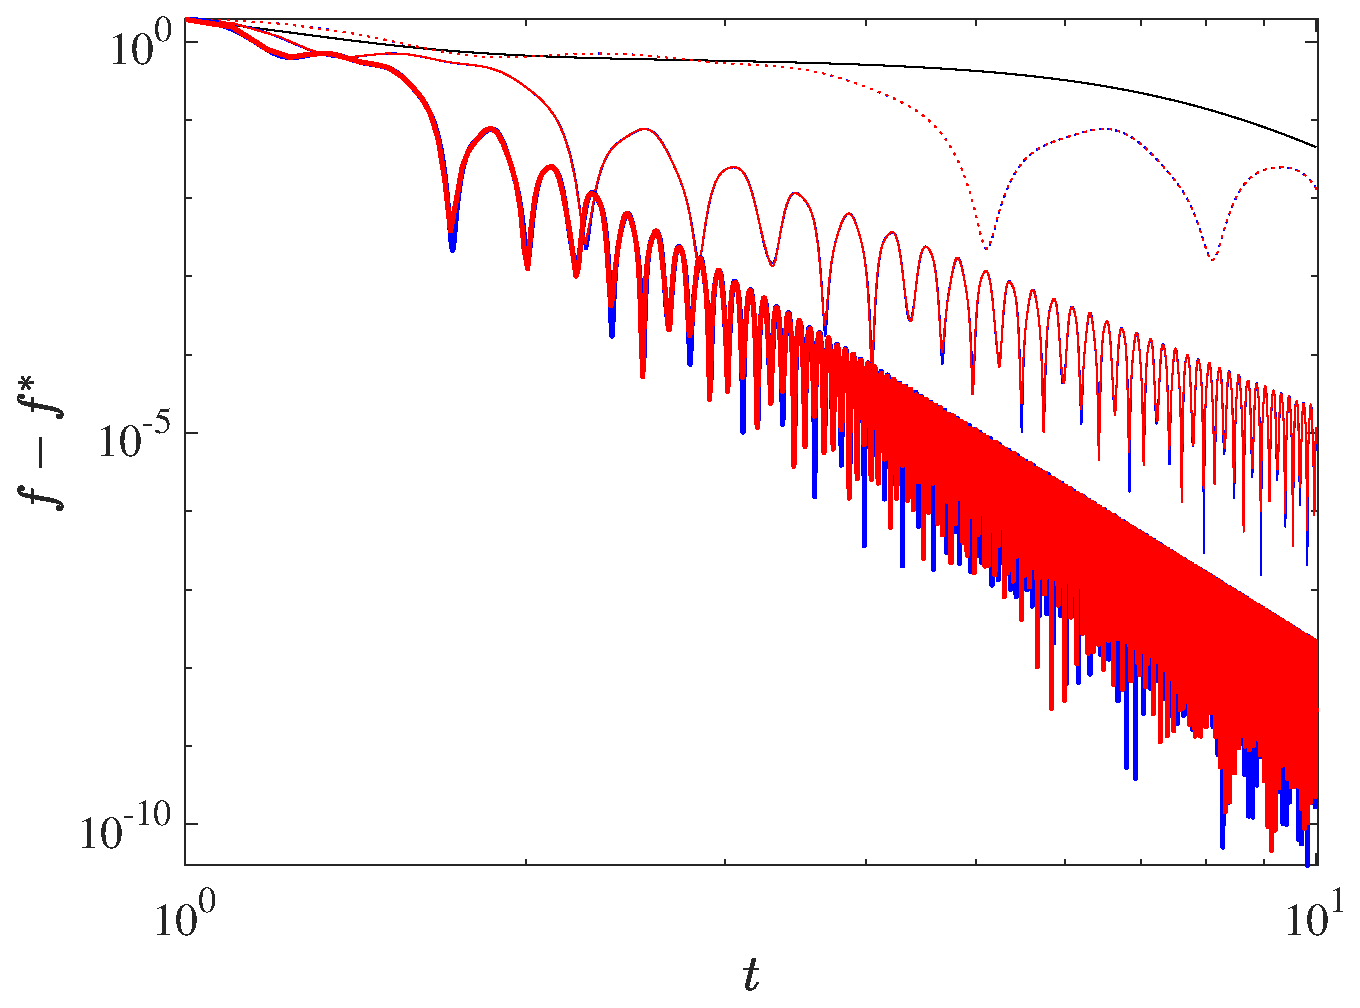
\includegraphics[width=0.7\columnwidth]{comp0_f}
        }
    }
    \centerline{
        \subfigure[Orthogonality error]{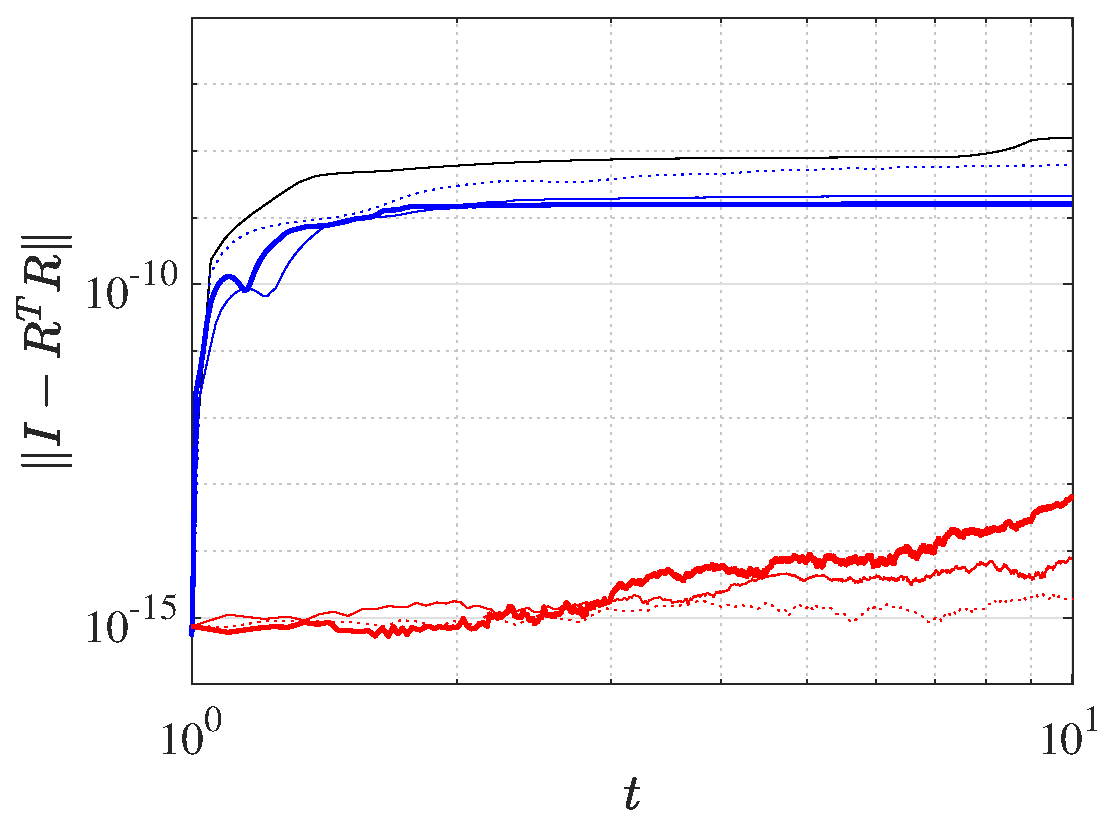
\includegraphics[width=0.7\columnwidth]{comp0_R}
        }
    }
    \caption{Simulation results: gradient descent (black); ode45 integration of continuous Bregman EL (red); LGVI (blue); $p=2$ (dotted); $p=4$ (thin); $p=6$ (thick)}\label{fig:1}
\end{figure}

\begin{thebibliography}{10}
\providecommand{\url}[1]{#1}
\csname url@rmstyle\endcsname
\providecommand{\newblock}{\relax}
\providecommand{\bibinfo}[2]{#2}
\providecommand\BIBentrySTDinterwordspacing{\spaceskip=0pt\relax}
\providecommand\BIBentryALTinterwordstretchfactor{4}
\providecommand\BIBentryALTinterwordspacing{\spaceskip=\fontdimen2\font plus
\BIBentryALTinterwordstretchfactor\fontdimen3\font minus
  \fontdimen4\font\relax}
\providecommand\BIBforeignlanguage[2]{{%
\expandafter\ifx\csname l@#1\endcsname\relax
\typeout{** WARNING: IEEEtran.bst: No hyphenation pattern has been}%
\typeout{** loaded for the language `#1'. Using the pattern for}%
\typeout{** the default language instead.}%
\else
\language=\csname l@#1\endcsname
\fi
#2}}

\bibitem{MarWesAN01}
J.~Marsden and M.~West, ``Discrete mechanics and variational integrators,'' in
  \emph{Acta Numerica}.\hskip 1em plus 0.5em minus 0.4em\relax Cambridge
  University Press, 2001, vol.~10, pp. 317--514.

\bibitem{LeeLeoCMAME07}
T.~Lee, M.~Leok, and N.~McClamroch, ``Lie group variational integrators for the
  full body problem,'' \emph{Computer Methods in Applied Mechanics and
  Engineering}, vol. 196, pp. 2907--2924, May 2007.

\bibitem{MarRat99}
J.~Marsden and T.~Ratiu, \emph{Introduction to Mechanics and Symmetry},
  2nd~ed., ser. Texts in Applied Mathematics.\hskip 1em plus 0.5em minus
  0.4em\relax Springer-Verlag, 1999, vol.~17.

\bibitem{LeeLeo17}
T.~Lee, M.~Leok, and N.~McClamroch, \emph{Global Formulation of {L}agrangian
  and {H}amiltonian Dynamics on Manifolds}.\hskip 1em plus 0.5em minus
  0.4em\relax Springer, 2018.

\bibitem{Leo04}
M.~Leok, ``Foundations of computational geometric mechanics,'' Ph.D.
  dissertation, California {I}nstittute of {T}echnology, 2004.

\bibitem{Lee08}
T.~Lee, ``Computational geometric mechanics and control of rigid bodies,''
  Ph.D. dissertation, University of Michigan, 2008.

\bibitem{tao2020variational}
M.~Tao and T.~Ohsawa, ``Variational optimization on lie groups, with examples
  of leading (generalized) eigenvalue problems,'' in \emph{International
  Conference on Artificial Intelligence and Statistics}, 2020, pp. 4269--4280.

\bibitem{wibisono2016variational}
A.~Wibisono, A.~C. Wilson, and M.~I. Jordan, ``A variational perspective on
  accelerated methods in optimization,'' \emph{proceedings of the National
  Academy of Sciences}, vol. 113, no.~47, pp. E7351--E7358, 2016.

\bibitem{nesterov2005smooth}
Y.~Nesterov, ``Smooth minimization of non-smooth functions,''
  \emph{Mathematical programming}, vol. 103, no.~1, pp. 127--152, 2005.

\bibitem{nesterov2008accelerating}
------, ``Accelerating the cubic regularization of newton’s method on convex
  problems,'' \emph{Mathematical Programming}, vol. 112, no.~1, pp. 159--181,
  2008.

\bibitem{duruisseaux2021variational}
V.~Duruisseaux and M.~Leok, ``A variational formulation of accelerated
  optimization on riemannian manifolds,'' \emph{arXiv preprint
  arXiv:2101.06552}, 2021.

\bibitem{alimisis2020continuous}
F.~Alimisis, A.~Orvieto, G.~B{\'e}cigneul, and A.~Lucchi, ``A continuous-time
  perspective for modeling acceleration in riemannian optimization,'' in
  \emph{International Conference on Artificial Intelligence and
  Statistics}.\hskip 1em plus 0.5em minus 0.4em\relax PMLR, 2020, pp.
  1297--1307.

\bibitem{WahSR65}
G.~Wahba, ``A least squares estimate of satellite attitude, {P}roblem 65-1,''
  \emph{SIAM Review}, vol.~7, no.~5, p. 409, 1965.

\end{thebibliography}

%\bibliography{/Users/tylee/Documents/BibMaster17,/Users/tylee/Documents/tylee}
%\bibliographystyle{IEEEtran}

\end{document}


